%% ****** Start of file aiptemplate.tex ****** %
%%
%%   This file is part of the files in the distribution of AIP substyles for REVTeX4.
%%   Version 4.1 of 9 October 2009.
%%
%
% This is a template for producing documents for use with 
% the REVTEX 4.1 document class and the AIP substyles.
% 
% Copy this file to another name and then work on that file.
% That way, you always have this original template file to use.

%\documentclass[aip,graphicx]{revtex4-1}
%\documentclass[aip,reprint]{revtex4-1}

%\usepackage{graphicx}

%\draft % marks overfull lines with a black rule on the right
%\documentclass[pre,aps,floatfix,authordate1-4,twocolumn]{revtex4-1}
%\documentclass[pre,aps,floatfix,authordate1-4]{revtex4-1}

\documentclass[aip,jcp,twocolumn]{revtex4}
%\documentclass[aip,jcp]{revtex4}
%\documentclass{article}



%\documentclass[aps,prl,preprint,groupedaddress]{revtex4}

\usepackage{rotating} 
\usepackage{times}
\usepackage{graphicx}
\usepackage{setspace}
\usepackage{amsmath}
\usepackage{epstopdf}
\usepackage[obeyFinal]{easy-todo}
\usepackage{csquotes}
\usepackage{mhchem}

%\usepackage{markdown} 

\begin{document}

% Use the \preprint command to place your local institutional report number 
% on the title page in preprint mode.
% Multiple \preprint commands are allowed.
%\preprint{}

\title{Accurate binding of calcium to phospholipid bilayers by effective inclusion of electronic polarization} %Title of paper

% repeat the \author .. \affiliation  etc. as needed
% \email, \thanks, \homepage, \altaffiliation all apply to the current author.
% Explanatory text should go in the []'s, 
% actual e-mail address or url should go in the {}'s for \email and \homepage.
% Please use the appropriate macro for the type of information

% \affiliation command applies to all authors since the last \affiliation command. 
% The \affiliation command should follow the other information.

\author{Josef Melcr}
\author{Hector Martinez-Seara Monne}
\author{Pavel Jungwirth}
\affiliation{Institute of Organic Chemistry and Biochemistry,
Academy of Sciences of the Czech Republic, 
Prague 6, Czech Republic}

\author{O. H. Samuli Ollila}
\email[]{samuli.ollila@helsinki.fi}
%\homepage[]{Your web page}
\affiliation{Institute of Organic Chemistry and Biochemistry,
Academy of Sciences of the Czech Republic, 
Prague 6, Czech Republic}
\affiliation{Institute of Biotechnology, University of Helsinki}


% Collaboration name, if desired (requires use of superscriptaddress option in \documentclass). 
% \noaffiliation is required (may also be used with the \author command).
%\collaboration{}
%\noaffiliation

\date{\today}

\begin{abstract}
  % insert abstract here
  \todo{Abstract directly from Joe's conference abstracts. To be rewritten.}
Classical molecular dynamics simulations give detailed information about membrane structure and dynamics. 
However, there is still a room for improvements in current force fields – it is known from the literature,
that the binding of ions, especially cations, to phopholipid membranes is overestimated in all classical models [1]. 
We suggest that the membrane-ion interactions can be corrected by including implicit electronic polarizability into the
lipid models through the electronic continuum correction (ECC) [2], which was already applied to monovalent and divalent
ions yielding models that feature correct ion pairing [3]. 
Using the electrometer concept [3, 4] and x-ray scattering form factors, our simulations point out that our hypothesis is
correct and ECC is indeed a missing important contribution in current classical lipid models. 
Moreover, the solid physical principles behind ECC are found not to hamper other relevant properties of a phospholipid bilayer. 
The new lipid model, "ECC-lipids", shows accurate binding affinity to sodium and calcium cations and head group order parameter response to bound charge. 
We also provide for the first time a realistic stochiometry of bound calcium cations to a POPC membrane, and their binding sites. 
This work will continue as an open collaboration project NMRlipids VI (http://nmrlipids.blogspot.fi).
\end{abstract}

%\pacs{}% insert suggested PACS numbers in braces on next line

\maketitle %\maketitle must follow title, authors, abstract and \pacs

% Body of paper goes here. Use proper sectioning commands. 
% References should be done using the \cite, \ref, and \label commands


% Here I write pseudo-article statements that will make the main argument.
% Beautiful polished sentences will be formed only afte we agree on these basic things
\section{Introduction}
Cation interactions with cellular membranes play a key role in several biological processes,
like in signal propagation in neurons and vesicle fusion.
\todo{JOE: list more introductory examples, where it has interesting effects.}
Zwitterionic phosphocholine (PC) lipid bilayers have been widely used as model systems
to understand molecular level details of specific cation interactions with
cellular membranes by using experimental \cite{cevc90,tocanne90,binder02,pabst07,uhrikova08}
and theoretical methods \cite{bockmann03,bockmann04,Berkowitz12,??} 
\todo{PAVEL: introduce previous theoretical work that discusses cation binding to POPC w.r.t. its specific moiteties, e.g. Lukas' paper}.
While relative binding affinity of different ions is agreed to follow Hoffmeister
series, the molecular details of binding and binding energetics are
not fully understood \cite{cevc90,tocanne90,seelig90,binder02,catte16,??}.
%General conclusion from experimental
%studies has been that multivalent ions and lithium have weak specific binding in
%phopholipid bilayers, while other monovalent ions do not essentially
%bind 
%The presence of anoinic lipids, like PS or PG,
%increase the concentration close to the bilayer and thus the amount of bound
%ions, but do not affect the specific binding constant \cite{seelig90}.
Non-invansive spectroscopic methods, like nucelar magnetic resosnance (NMR), scattering
and infrared scpectroscopy, give accurate information about ion binding
in lipid bilayers\cite{hauser76,hauser78,herbette84,akutsu81,altenbach84,binder02}. 
Molecular level interpretation of the results, however, requires assumptions
about binding models and is often not fully conclusive \cite{??}.
On the other hand, the accuracy of the state of the art atomistic resolution lipid and ion models
have turned out insufficient for the detailed interpretation of cation binding details \cite{catte16}.
The overestimated specific cation binding observed in current lipid models \cite{catte16}
may lead to articifially positively charged memranes and significant artefacts in
MD simualtions (e.g.~divalent cation-induced charge inversion of bacterial membranes~\cite{Luan2016}
\todo{JOE: this may be a too daring statement. \\
  SAMULI: I think that the divalent cation induced charge inversion is not an artefact,
  but it might happen with too small concentrations. 
  On the other hand, it is not a new observation either, see e.g. literature cited in NMRlipids IV project.}). 

%The binding details, like binding sites and stoichiometry are not yet fully
%resolved but interpretation of NMR and scattering experiments suggest that one
%Ca2+ interacts mainly with the choline groups \cite{hauser76,hauser78,herbette84} of two
%phospholipid molecules \cite{altenbach84}.

In this work we show that the accuracy of ion binding, especially calcium,
in zwitterionic PC lipid bilayer can be significantly improved 
for classical MD simulation models of zwitterionic lipids
by including electronic polarizability
in the polar region of lipid molecules
using the electronic continuum correction (ECC)~\cite{leontyev11}. 
This approach has been previously shown to improve performace of
ion models against neutron scattering data in concentrated solutions 
and ab-initio simulations~\cite{Jungwirth2017,Jungwirth2015,kohagen14,kohagen16}. 
The realistic structure of ions in a bulk solvent was not, however, sufficient to correct binding in lipid
bilayers~\cite{catte16}. 
To fix it, we propose
a classical fixed-charge MD simulation model of 
1-Palmitoyl-2-oleoylphosphatidylcholine (POPC) lipid 
that accounts for electronic polarizability by using ECC. 
We will validate such a model by comparing its lipid bilayer structue
to x-ray scattering data and its head group structure to NMR experiments. 
We will then quantify the accuracy of the head group order parameter response to the bound charge
and compare it to the experimental NMR data of sodium and calcium binding in PC lipid bilayers. 
In addition, we will quantify relative binding affinities of different moieties in POPC to such cations. 
This will be discussed in terms of binding modes, stoichiometry and binding isotherms and their models used in experiments.
The proposed POPC model, ECC-lipids, and the approach to obtain it
is, hence, highly useful for future MD simulations with physiological salt conditions, 
and for effects where membrane electrostatics play a major role.




\section{Methods}

\subsection{Electronic continuum correction for lipid bilayers}\label{section:ecc}
The lack of electronic polarizability in the standard MD simulation
force fields has been considered higly relevant issue since the early days of
lipid bilayer simulations.
%Some pioneering simulation studies scaled
%the partial charges of atoms by one half to effectively include 
%polarizability \cite{jonsson86,egberts94}. Also, approaches that
%explicitly include polarizability has been introduced, but
%this has turned out to be practically complicated \cite{chowdhary13}.
In this work we circumvent the rather demanding explicit inclusion
of electronic polariization effects \cite{chowdhary13} by effectively including
electronic polarizability in lipid
bilayer simulations by using the electronic continuum correction
(ECC)~\cite{leontyev11}. 
Technically, it is a similar approach to the phenomenological charge-scaling as applied in 
the early studies where a scaling factor one half was used \cite{jonsson86,egberts94}. 
However, the concept of ECC is 
physically well justified and rigorously derived~\cite{leontyev09, leontyev10, leontyev11},
but significantly more simple than the explicit inclusion of electronic
polarizability \cite{chowdhary13} both for derivation and application.


According to ECC, electronic
polarizability can be included in classical MD simulations by
placing all particles into a homogeneous dielectric continuum 
with a dielectric constant $\epsilon _{el}$, 
which is the electronic part of the dielectric constant of 
the media \cite{leontyev11}. Measurements of high frequency 
dielectric constant gives values of approximately $\epsilon _{el} \approx 2$ 
for almost any biomaterial \cite{some_original_work, leontyev11}.
Such a dielectric continuum can be easily included in standard MD simulation by
a formal transformation of partial charges 
\begin{equation}
  Q^{ECC} = f_q \cdot Q
\end{equation}
with a constant scaling factor $f_q = \epsilon _{el} ^{-1/2}$ 
effectively representing the newly introduced electronic continuum. 
The value measured for water, $\epsilon _{el} = 1.78$, gives 
a scaling factor of $f_q = 0.75$ \cite{some_orig_source, leontyev11}, which has been
successfully used to improve the performance of force field for ions \cite{kohagen14,kohagen16,??}. 

While the scaling factor of $f_q = 0.75$ for ions in water is well justified and 
improves model performance against experimental scattering data \cite{kohagen14,kohagen16, Pluharova2014},
it is not clear if the same factor should be used for partial charges in molecules,
i.e, lipids in our case. Unlike the total charge of ions, atomic partial charges in
classical MD simulations are not experimental observables.
Instead they are based on theoretical calculations and the
derived values depend, for example, on the conformational
sampling of the molecules and description of solvent 
in the calculations \cite{RESP_paper,??}. 
%In cases where the partial charges have some physical meaning 
%(e.g. approximate electrostatic potential as in RESP~\cite{RESP_paper}),
Depending to the details, partial charge calculations may partially
include some of the solvent electronic polarizability effects. Thus, we expect that
the correct ECC scaling factor, $f_q$, for molecular partial charges would lie
between $\epsilon _{el} ^{-1/2}$ (no electronic polarizability in charge calculation)
and $1$ (full electronic polarizability in charge calculation).

In this work, we empirically sample this parameter space
to find a atomistic MD simulation force field parameters for lipids that
accurately describe the lipid head group response to Na$^+$ and Ca$^{2+}$ concentrations
when compared with NMR data \cite{akutsu81,altenbach84}. This data can be used to accurately asses
ion binding in PC bilayers, as discussed in Ref, \citenum{catte16} and in section \ref{section:electrometer}.
We chose the Lipid14~\cite{dickson14} force field parameters as a starting point,
because their response to bound ions was apparently most realistic against NMR data
in recent work by NMRlipids project (see Fig.~5 in Ref.~\citenum{catte16}).
Also glycerol backbone and head group structures in Lipid14 model were
relatively realistic when compared with other state of the art lipid models \cite{botan15}.
The ECC correction was applied to Lipid14 parameters by scaling partial charges of the headgroup,
glycerol backbone and carbonyl regions, which are the most polar parts in lipids and
are expected to have the largest contribution to the cation binding.
The hydrocarbon chain parameters are not modified, because they are
already highly optimized and give generally a good description for
hydrophobic part of lipid bilayers in various conditions
in most lipids models, including Lipid14 \cite{ollila16}.
In contrast, improvements in glycerol backbone and headgroup
parameters are required in all available lipid models~\cite{botan15}. 

Exploring different scaling factor values, applied to headgroup, glycerol backbone
and carbonyl charges of Lipid14 model, we found out that ion binding and
related headgroup order parameter response became weaker with the scaling of partial
charges. The optimal behaviour of ion binding was observed with
the scaling factor $f_q = 0.8$. % is optimal for applying ECC on Lipid14 model. 
Interestingly, this scaling factor is in line with the estimate
given by ``implicitly polarized charges'' (IPolQ) \cite{ipolq2013}
combined with RESP calculations in vacuum and implicit solvent reported
in \cite{maciejewski14}. IPolQ charges are obtained as the average of
partial charges given by RESP calculation~\cite{RESP_paper}
in vacuum and in a solvent. Applying the scaling factor of 0.75 to
IPolQ charges calculated from the data in Ref.~\cite{maciejewski14},
gives similar partial charges to ones obtained by scaling Lipid14 charges
with a factor 0.8.
%-----\footnote----------
  %{Depending on which QM method you arrive at values from 0.76 to 0.83, averages across atom
  %types being around 0.78--0.80. Even though the methods are almost identical, authors of Lipid 14 find lower
  %partial charges in vacuum than here -- so I prefer the higher value. As the choice of charges is arbitrary anyway,
  %I use 0.80 as an approximate round value, which accounts for the already lower charges in Lipid14. 
  %The use of 0.78---.79 might be more appropriate, though.}


While, the charge scaling improved the behaviour of lipid-ion interactions,
it reduced the area per molecule of lipid bilayer without ions below experimental
values. Simulations with Lipid14 parameters having partial charges of headgroup, glycerol
backbone and carbonyls scaled with 0.8 gave the area per molecule value of $\approx$60~\AA$^2$,
which is significantly smaller than the experimental value 64.3~\AA$^2$ (\cite{}\todo{missing REF for APL experiment})
and the original Lipid14 value $(65.6 \pm 0.5)$~\AA$^2$~\cite{dickson14}.
The decrease of area was found to arise from a lower hydration of the lipid head group region,
which can be explained by the decreased solvation free energy due to the lower polarity
of molecules with scaled charges. The hydration can be increased
by reducing the effective radius of atoms by changing the 
the $\sigma$ parameters in Lennard-Jones potential for the selected atoms
similarly as done for free ions in solution \cite{kohagen14,kohagen16,??}.
This increases solvation free energy by allowing water molecules to
approach closer to lipid atoms and have stonger electrostatic interactions with them.
After reducing the $\sigma$ parameters with a factor of $f_\sigma = 0.89$
for the same atoms for which charges were scaled, the area per molecule value was
again in agreement with experimental value (see Table~\ref{tab:apls}). 


\subsection{Comparison of ion binding affinity to experiments by using the electrometer concept} \label{section:electrometer}
Ion binding was compared between experiments and simulations by 
using lipid head group order parameters and ''electrometer concept'' 
introduced by Seelig et al. \cite{seelig87,catte16}.
The concept is based on the experimental observation that the 
order parameters of $\alpha$ and $\beta$ carbons in lipid head group
(see Fig. \ref{??} 
\todo{Figure with chemical structure and labeling to be added}) 
are proportional to the amount of bound charge
in lipid bilayer \cite{seelig87}.
More recent analysis included also
the order parameter signs and concluded that the order parameters  
decrease with bound positive charge and increase with bound negative 
charge \cite{ollila16,catte16}. The observations are rationalized 
as a change of lipid head group dipole tilt to more vertical orientation
with bound positive charge and {\it vice versa} for negative charge \cite{seelig87}. 
Order parameters for $\alpha$ and $\beta$ segments in headgroup, as well as for
all C-H bonds in lipid molecules,
can be accurately measured by using H$^2$ NMR or $^{13}$C NMR techniques.
The experimental order parameters can be compared with the the ones
calculated from MD simulations by using the definition
\begin{equation}\label{OP}
S_{\rm CH}=\frac{3}{2}\langle \cos^2\theta -1 \rangle,
\end{equation}
where $\theta$ is the angle between the bond and membrane
normal and average is taken over all sampled configurations \cite{ollila16}.

According to the electrometer concept,
the change of the head group order parameters as a function of
the amount of bound charge per lipid $X^\pm$ 
can be written as~\cite{ferreira16}
\begin{equation}\label{OPchangeEQ}
\Delta S_{\rm{CH}}^{i}= S_{\rm{CH}}^{i}(X^\pm)-S_{\rm{CH}}^{i}(0) =\frac{4m_i }{3\chi}X^\pm,
\end{equation}
where $S_{\rm{CH}}^{i}(0)$ denote the order parameter in the absence of bound charge,
$i$ refers to either $\alpha$ or $\beta$ carbon,
%the empirically observed linear relation %for the change in order parameters %with respect to a bilayer without bound charges              
%\begin{equation}\label{electrometer_eq}                                                                                                   
%S_{\rm{CH}}^{i}(X^\pm)=S_{\rm{CH}}^{i}(0) + \frac{4m_i}{3\chi} X^\pm,                                                                     
%\end{equation}                                                                                                                            
$m_i$ is an empirical constant depending on the valency and position of bound charge,
and the value of the quadrupole coupling constant is $\chi \approx$\,167\,kHz.
Atomic absorption spectra and $^2$H NMR data, combined with the
information about order parameter signs gave
$m_\alpha=-20.5$  and $m_\beta=-10.0$ for Ca$^{2+}$ binding to POPC
bilayer (in the presence of 100~mM NaCl)~\cite{altenbach84,ollila16,catte16}.
Recent work published by the NMRlipids project showed that the concept works
qualitatively also in simulations and can be used to compare ion binding
affinitity between simulations and experiments~\cite{catte16}.

The experimental data used to quantify cation binding reports
order parameters as a function of equilibrium cation concentration
in the bulk solvent \cite{akutsu81,altenbach84}. Recent work
by NMRlipids project estimated this concentration by using
the relative molar concentration in water
[salt]=N$_{\rm c} \times$[water]\,/\,N$_{\rm w}$, where [water]\,=\,55.5~M,
which was accurate enough for the conclusions in that study \cite{catte16}.
Since we are now targeting a model with quantitatively accurate binding
affinity, we used larger simulation box dimensions that allow the
determination of bulk ion conceration. Equilibrium concentration
corresponding the experimental data in the units of $\mathrm{mol/l}$
can be then determined from the ion concentration plateau in the bulk s
olvent at the boundaries of the simulation box as
\begin{equation}
\label{eq:conc}
  C_{eq}=\frac{C_{plateau}}{0.602},
\end{equation}
where plateau concentration is the number density in the units of $\mathrm{nm}^{-3}$.
\todo{SAMULI: Once we have to final results, we can probably say that
  the repeat distance is not far from the experimentally measured distance \cite{pabst07,uhrikova08}
  }

The ion binding affinities between different models were compared by calculating
the relative surface excess between water and ions $\Gamma_w^i$ \cite{chattorajBOOK}
\begin{equation}
  \Gamma_w^i=\Gamma_w^x-\Gamma_i^x\frac{c_w-c_w'}{c_i-c_i'},
\end{equation}
where $c_w$ and $c_i$ are concentrations in bulk water, 
$c_w'$ and $c_i'$ are concentrations inside bilayer, and
$\Gamma_w^x$ and $\Gamma_i^x$ are surface excess of water and
ions, respectively. The whole simulation box is considered here
as interfacial region, thus $\Gamma_w^x=n_w/A$ and $\Gamma_i^x=n_i/A$,
where $A$ is the area of the simulation box, and $n_w$ and
$n_i$ are total number of water and ions in simulation box,
respectively. The concentrations of water and ions inside
bilayer can be expected to vanish, thus $c_w'=c_i'=0$.
Then we get the relative surface excess for lipid bilayer
simulations
\begin{equation}\label{surfexcess}
  \Gamma_w^i=\frac{n_w}{A}-\frac{n_i}{A}\frac{c_w}{c_i},
\end{equation}
where concentrations in bulk, $c_w$ and $c_i$, can be determined
from the simulation box boundary.

\subsection{Comparison of lipid bilayer structure to experiments}

Lipid bilayer structure without ions was validated against NMR experiments
by order parameters for C-H bonds and x-ray scattering experiments by using
form factors. The former validates the structures sampled by individual
lipid molecules in simulations with segmental resolution, while the latter
validates the dimensions of the lipid bilayer (thickness and area per
molecule)~\cite{ollila16}.

Order parameters were calculated from simulations for all C-H bonds
by using Eq. \ref{OP} and form factors as
\begin{equation}
  F(q) = \int _{-D/2} ^{D/2} \left ( \sum _\alpha f_\alpha (q_z) n_\alpha (z) - \rho _s \right ) \exp (izq_z) \mathrm{d}z,
\end{equation}
where $f_\alpha(q_z)$ is the density of atomic scattering length, 
$\rho_s$ is the density of solvent scattering lenght,
$n_\alpha (z)$ is the number density of atom $\alpha$ and
$z$ is the distance from the membrane centre along its normal 
spanning the membrane with thickness $D$. 




\subsection{Simulation details}

\subsubsection{Simulations with aqueous ions}
The simulated systems consisted of 1-Palmitoyl-2-oleoylphosphatidylcholine
(POPC) bilayer and an aqueous salt solutions of varying concentrations.
Water molecules were described by OPC3 model \cite{Izadi16}
\todo{Explain why were OPC3 chosen}.
In order to test transferability of the newly developed ECC-lipids model, 
we also performed several additional simulations with water models 
OPC \cite{Izadi14}, SPC/E \cite{Berendsen1987} and TIP4p/2005 \cite{Abascal2005}
presented in Supporting Information (SI). 
We used ECC-ions model for ions \cite{jungwirth17-new-paper-to-be-published, kohagen16, Pluharova2014}.  % cite order: [Ca_2s, Na_s, Cl_2s]
Simulations with Lipid14 use ion model by Dang \cite{smith94,chang1999,dang2006}. 
Classical molecular dynamics simulations were performed using the GROMACS \cite{Abraham15} simulation package (version 5.1.4).  
The simulation settings used in this work are 
summarized in Table \ref{tbl:mdpar}, 
and they are based on previously used settings in \cite{catte16} available at \cite{lipid14POPC0mMNaClfiles}. 
Simulation trajectories and parameters are available at \cite{??} \todo{To be uploaded to Zenodo}. \\
\todo{System sizes has to reported somewhere}

\begin{table}[btp]
  \caption{Simulation parameters}
  \label{tbl:mdpar}
  \begin{tabular}{ll}
    simulation property & parameter   \\
    \hline
    time-step           & 2~fs         \\
    equilibration time  & 100~ns  \\
    simulation time     & 200~ns  \\
    temperature         & 313~K       \\
    thermostat          & v-rescale  \cite{bussi07}   \\
    barostat            & Parrinello-Rahman, semi-isotropic \cite{parrinello81} \\
    long-range electrostatics & PME  \cite{darden93}  \\
    cut-off scheme      & Verlet \cite{Pall13}      \\
    Coulomb and VdW cut-off & 1.0~nm \\
    constraints         & LINCS, only hydrogen atoms \cite{hess97} \\
    constraints for water & SETTLE  \cite{miyamoto92} \\
    \hline
  \end{tabular}
  \todo{This could be moved to SI. Only simulation lengths needs to be mentioned in the main paper.}
\end{table}


\subsubsection{Simulations with cationic surfactants}
Automated topology builder \cite{malde11} was first used to create the structure of
dihexadecyldimethylammonium bromide, C$_{12}$Cl$_{16}$$^+$N2C$_1$Br$^-$, molecule.
AmberTools program \cite{amber} was then used to generate the Amber-type force field
parameters. The parameters were converted to the Gromacs format by using
acpype tool \cite{acpype}. The partial charges were then manually modified
to approximately correspond to their equivalent segments in Lipid14 \cite{dickson14}.
The surfactants were randomly placed among the lipids to form bilayer structures with
mole fractions 10\%, 20\%, 30\%, 42\% and 50\% of surfactant in the POPC bilayer.
All systems contained 50 POPC molecules per leaflet, 6340 TIP3P water molecules and
6, 14, 21, 35 or 50 surfactants per leaflet.
These systems were first simulated 200~ns by using Lipid14 model.
First 20~ns was omitted from the analysis. 

The same systems where also simulated with ECC-corrected lipi model...
\todo{Describe the changes in surfactant model used with ECC-corrected lipids.}

\section{Results and Discussion}

\subsection{POPC membrane and its structure}

\begin{figure}[tbp]
  \centering
  \includegraphics[height=8.5cm,angle=-90]{../Fig/form-f_exp-l14-eccl17.eps}
  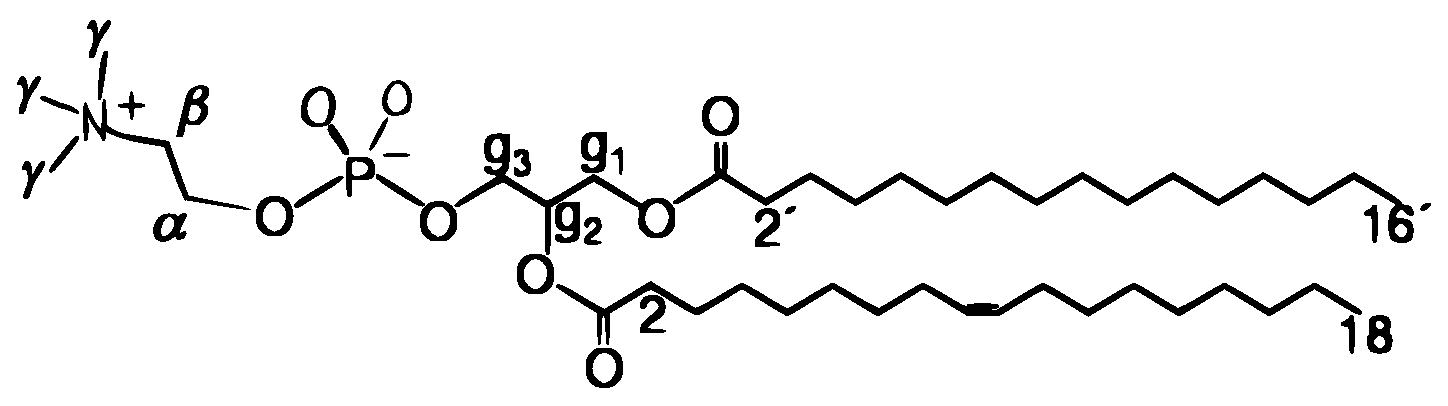
\includegraphics[width=7.0cm]{../Fig/POPCstructure.eps}
  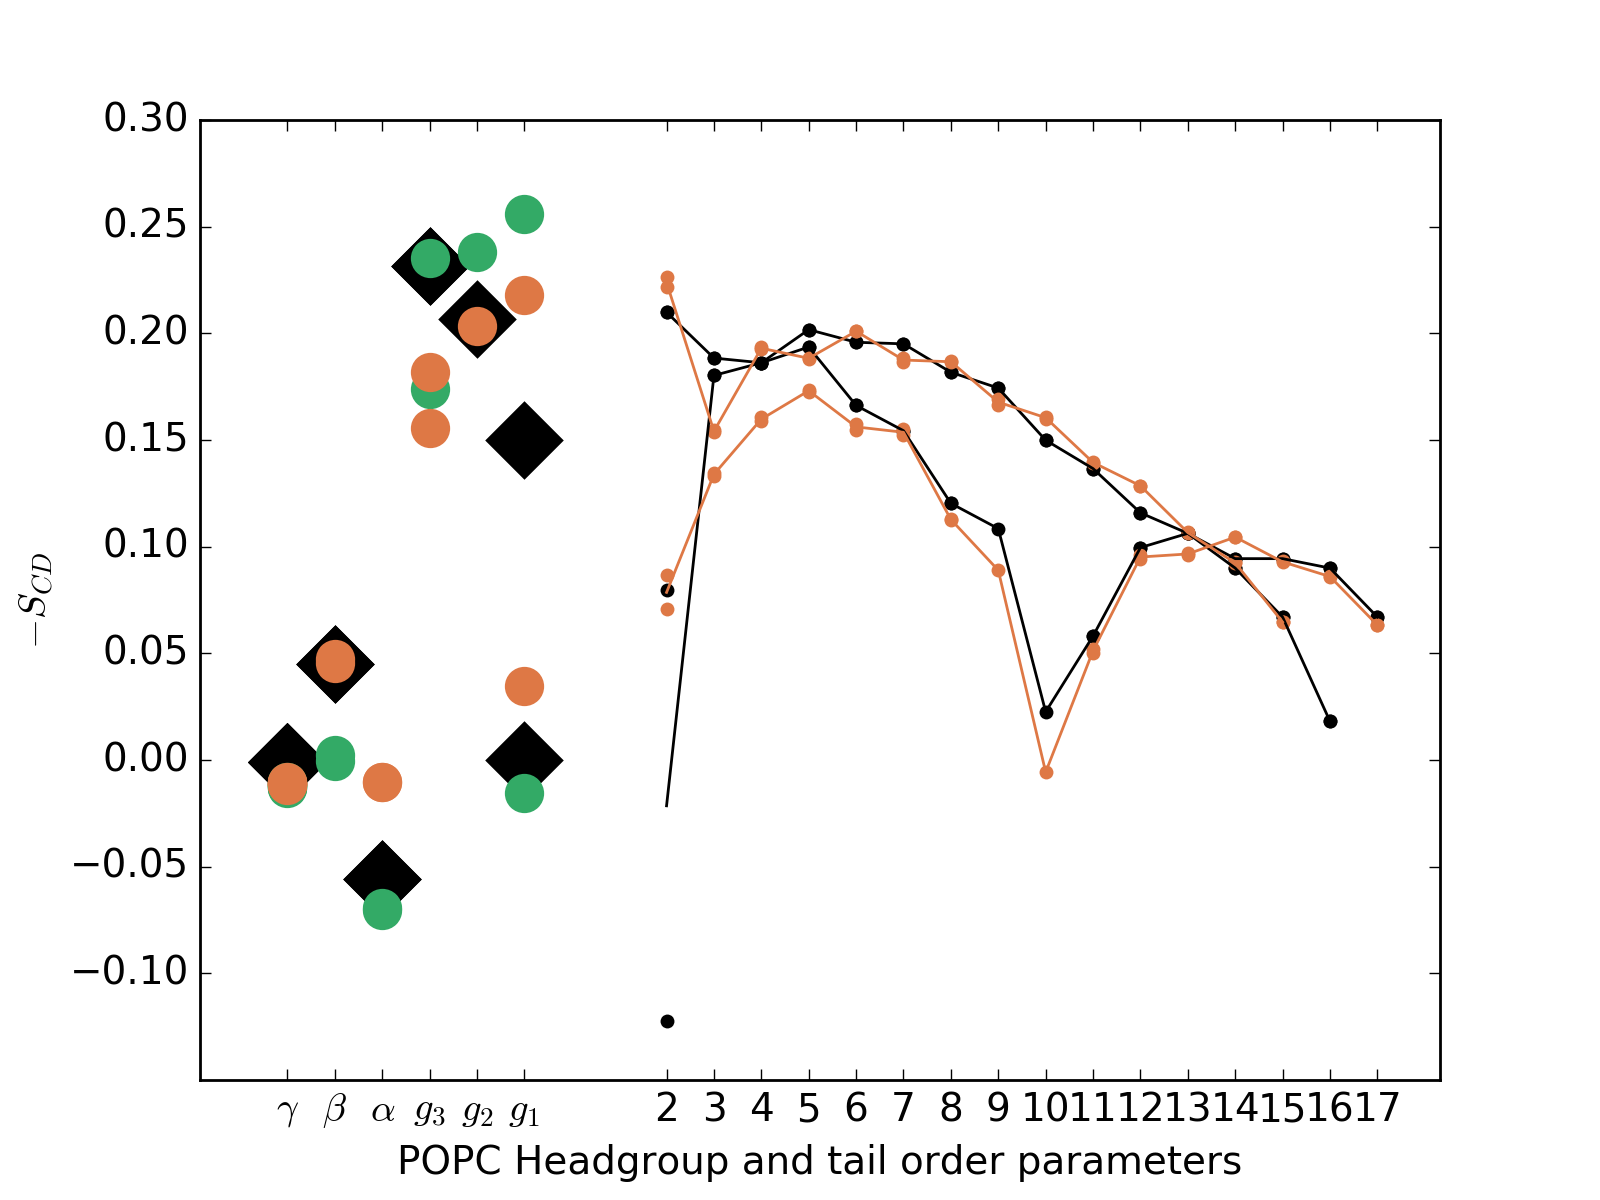
\includegraphics[width=9.0cm]{../Fig/ipython_nb/Order-parameters_exp-L14-ECCL17_q80_sig89.png}
  \caption{\label{simVSexpNOions}
    X-ray scattering form factors from experiments~\cite{Kucerka2011} and simulations using Lipid14 \cite{dickson14} and ECC-lipids models. 
    Order parameters of head group, glycerol backbone and sn-1 and sn-2 tails  from simulations with Lipid14 \cite{dickson14} and ECC-lipids models
    compared with experimental order parameters from \cite{ferreira13}.}
  \todo{We should run a simulation for the system withtout ions with the
    same (or close) temperature as the experimental data. The NMR data is at 300K
    so that would be good. I think that this would be also close enough for the scattering data at 303K.
  }
\end{figure}

\begin{table}
  \caption{Area per lipid (APL) from different models of POPC without ions\label{tab:apls} }
  \begin{tabular}{l|c c}
    model          & APL (\AA$^2$)   & Temperature [K] \\
    \hline
    Lipid14 \cite{dickson14}  & 65.6$\pm$ 0.5  &  303 \\
    \hline
    ECC-lipids &        &  \\
    %Lipid14ecc0.80+sigma0.875 &        &  313    \\
    ($4.6\cdot 5.1 \, \mathrm{nm}^2$), 72 lipids patch, OPC3           & 63.2   &   313      \\
    \hline
    (6.4 nm)$^2$, 128 lipids patch, OPC3           & 64.2   &  313       \\
    (6.4 nm)$^2$, 128 lipids patch, SPC/E          & 65.1   &  313       \\
    (6.4 nm)$^2$, 128 lipids patch, OPC            & 64.4   &  313       \\
    (6.4 nm)$^2$, 128 lipids patch, TIP4p/2005     & 66.8   &  313       \\
    %($9.2\cdot 10.2 \, \mathrm{nm}^2$), 288 lipids patch           & 65.5   &  313       \\ %% not done for this model with f_sigma=0.89
    %oMM small patch           & 63.65  &         \\
    %oMM 4xbig patch           & 63.7   &         \\
    \hline
    %experiment   & 62.7  &  293    \\
    experiment \cite{jambeck12}\todoii{REF}{put original references, not Slipids param. paper.} & 64.3  &  303    \\
    experiment  & 67.3  &  323    \\
    %experiment  & 68.1  &  333    \\
    %experiment POPE  & 56.6 &  303    \\
    \hline
  \end{tabular}
\end{table}


In order to validate the newly developed model, ECC-lipids, 
we compared our simulation results without any ions to
NMR order parameters measurements and x-ray scattering form factors 
(Fig.~\ref{simVSexpNOions} and Table~\ref{tab:apls}). 
The tail order parameters being already highly optimized in the original Lipid14 model~\cite{dickson14}
are found to match the experimental values nicely.
The head group and glycerol backbone order parameters accuracy is 
comparable to the state of art lipid models available in literature \cite{ollila16}.
The agreement between the x-ray scattering form factors and the areas per molecule from simulations and experiments
confirm that the membrane structural properties are well captured. 
A structural comparison of ECC-lipids with Lipid14 can be found 
in SI along with results with other water models. 
%The optimal value for $f_\sigma$ was found by representing the overall membrane structure well
%by matching scattering form factors to experimental data~\cite{Petrache06, Kucerka08, Pabst10}.

\subsection{Response of POPC headgroup on bound charge}

\begin{figure}[tbp]
  \centering
  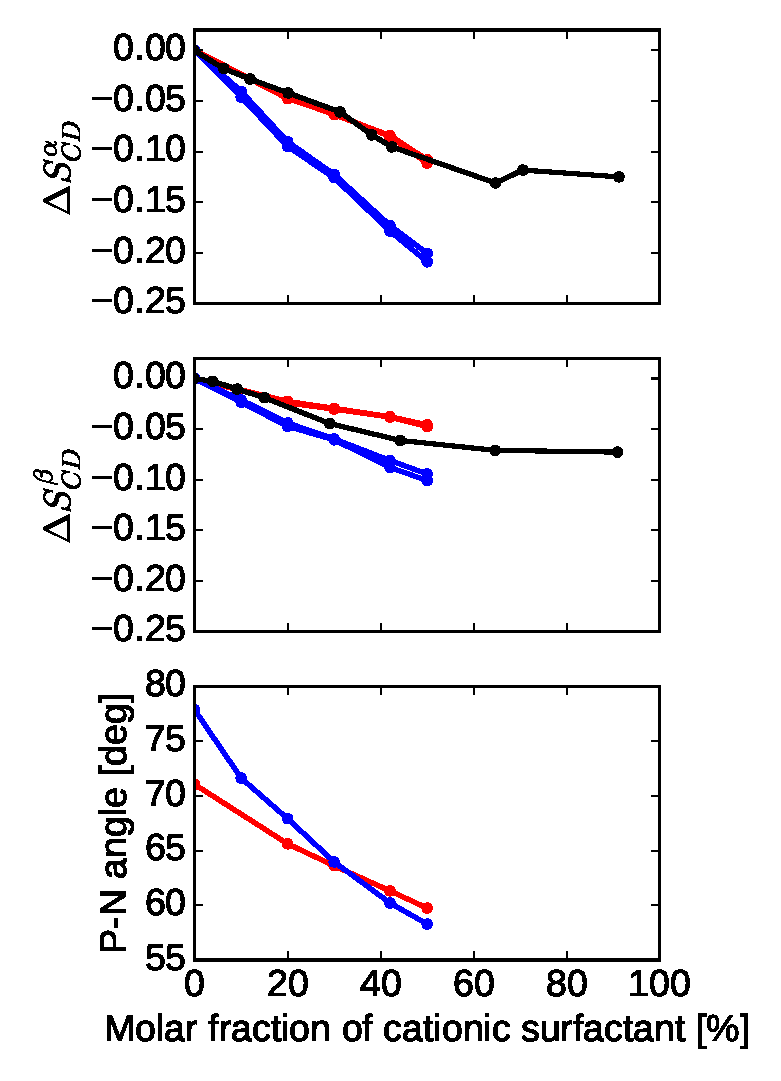
\includegraphics[width=8.0cm]{../Fig/ipython_nb/PN_angle_OrdPars-A-B_L14-ECCL17_q80_sig89_surf.eps}
  \caption{\label{OrderParameterCHANGESsurf}
    Headgroup order parameter changes and P-N vector orientation as a function of
    cationic surfactant (dihexadecyldimethylammonium bromide, C$_{12}$Cl$_{16}$$^+$N2C$_1$Br$^-$)
    in PC bilayer from simulations and experiments \cite{scherer89}.
  }
  \todo{Labels are missing.} \\
  \todo{Order should be the same as in other figures, i.e, $\beta$ segment on top.} \\
  \todo{I would put x-axis from 0 to 51 and maybe zoom y-axis little bit as well.}
\end{figure}

The headgroup response to bound charge depends on both, the
binding affinity and the response of the headgroup on bound charge.
Thus, the headgroup response to bound charge has to be correctly
described in the model if the concept is used for quantitative studies of
binding affinity. Hence, we first quantify the response of head group order
parameters to the bound charge by using experimental data measured from
mixtures of cationinc surfactants and PC lipids~\cite{scherer89}.
The amount of the bound charge is known excatly in these systems,
because essentially all surfactants with unit charge locate in lipid bilayers.
%Thus, the headgroup order parameter response to bound charge can be first
%quantified aginst experimental data before proceeding to binding affinity studies.
%Headgroup order parameter response to the amount of bound charge can
%be quantified by using ionic surfactants with a known valency~\cite{scherer89}.
%All surfactants locate in lipid bilayers due to their amphiphilic nature,
%thus the exact amount of bound charge in the membrane is known in these systems.
%The headgroup order parameter changes as a function of bound charges can be then
%explicitly determined from such systems.

Changes of headgroup order parameter as a function of added cationic surfactant
dihexadecyldimethylammonium bromide (C$_{12}$Cl$_{16}$$^+$N2C$_1$Br$^-$) from
experiments~\cite{scherer89} and simulations are shown in
Fig. \ref{OrderParameterCHANGESsurf}).
As expected from Eq. \ref{OPchangeEQ}, the head group order parameter response to the bound cation concentration
is approximately linear at least up to $\sim$0.3 mole fraction in experiments and
in both simulation models, original Lipid14 and ECClipids \todo{Yet to be shown.}. 
\todo{We might want to calculate the slopes from simulations.}

The slope is, however, too steep in Lipid14 model indicating that the
headgroup order parameters are too sensitive for bound charge in this model.
This has to be taken into account when interpreting the
headgroup order parameter response to CaCl$_2$ concentration in Lipid14 model.
%observed in  Ref. \citenum{catte16}, see also Fig. \ref{OrderParameterCHANGESnewMODELS}.
The ECC-lipids model gives a slope in very good agreement with experiments
for the $\alpha$ segment, while the slope is slightly
underestimated for the $\beta$ segment.
%The present comparison of head group order parameter changes 
%suggests that the observed overestimated response of all models to 
%increasing CaCl$_2$ concentration in \cite{catte16} 
%can be explained at least in part by a high sensitivity of the head group order parameter response
%to the bound charge.

Also the angle of the headgroup P-N vector with respect to membrane normal
is shown in Fig.~\ref{OrderParameterCHANGESsurf} as a function of bound cations.
As expected~\cite{seelig87}, the headgroup orients more parallel with membrane
normal with increasing amount of bound cations. The effect is stronger
in Lipid14 parameters than in ECClipid parameters, which is in line
with the reduced dipole moment and the lower sensitivity to bound charges
in the ECClipid model.
\todo{It might be a good idea to establish a relation between order parameter change
and P-N vector angle by using ECClipids model.}


\subsection{Cation binding affinity in POPC}

\begin{figure*}[tbp]
  \centering
  \includegraphics[width=16.0cm]{../Fig/OrdParChanges_NaCl_CaCl2.eps}
  \caption{\label{OrderParameterCHANGESnewMODELS}
    Headgroup order parameter changes as a function of NaCl, CaCl$_2$ concentration
    from simulations with different force fields and experiments (DPPC \cite{akutsu81} and POPC \cite{altenbach84}).
    Simulations with Lipid14 parameters and Aqvist ions are directly from Ref. \cite{catte16}, except that
    the concentration are determined with Eq. \ref{eq:conc}.
  }
  \todo{Simulation results with original Slipids and Dang ions to be added when we have the results.}
\end{figure*}


%After achieving accurate head group order parameter response with a cationic surfactant, 
%we advanced to quantifying the response to solutions with varying concentrations of salts, namely \ce{NaCl} and \ce{CaCl_2}.
The headgroup order parameter response to aqueous ionic concentration
can be used to measure ion binding affinity in experiments and simulations,
as discussed in section \ref{section:electrometer} and in previous literature~\cite{seelig87,catte16}.
The headgroup order parameter response of PC lipids to NaCl and CaCl$_2$ concentrations
from experiments (DPPC \cite{akutsu81} and POPC \cite{altenbach84}) and different simulation
models are shown in Fig. \ref{OrderParameterCHANGESnewMODELS}.
The simulation results of Lipid14 with Aqvist ions \cite{??} (from Ref. \citenum{catte16})
are shown together with the results from Lipid14 simulation
with Dang ions \cite{??} and from ECClipid simulations with ECC-ions.

As already discussed in the recent work by NMRlipids project~\cite{catte16},
the headgroup order parameters are almost unaffected by addition of NaCl
in Lipid14 simulations with Aqvist ion model due a very weak binding of Na$^+$
in PC bilayer. This is in agremeent with experimental data, in contrast
to almost all the other lipid models, which significantly overestimate
Na$^+$ binding in PC bilayers~\cite{catte16}. Despite of good performance
with NaCl, the response of headgroup order parameters to CaCl$_2$ concentration are
significantly overestimated in Lipid14 simulations with Aqvist ion model,
see Fig.~\ref{OrderParameterCHANGESnewMODELS} and \citenum{catte16}.

Wide range of data presented in previous work \cite{catte16} suggested
that CaCl$_2$ binding behaviour cannot be corrected by only improving
ion models. This was not, however, tested for Lipid14 model, so we
ran also Lipid14 simulations with Dang \cite{smith94,chang1999,dang2006} and ECC corrected \cite{??}
ions having more realistic bulk behaviour as Aqvist model \cite{??}.
In line with previous work, the headgroup order parameters response
to CaCl$_2$ concentartion was overestimated also with these ion models,
as seen in Figs. \ref{OrderParameterCHANGESnewMODELS} and \ref{??} (in SI), respectively
\todo{Add OP-response of Lipid14+Dang in Fig. \ref{OrderParameterCHANGESnewMODELS}
  and OP-response of Lipid14+ECC-ions plot in SI}.

Applying ECC correction also for lipids, introduced in section \ref{section:ecc},
brings the order parameter response to CaCl$_2$ concentration to a
good agreement with experiments, as shown in Fig. \ref{OrderParameterCHANGESnewMODELS}.
This is a significant improvement over previously introduced models,
which all overestimate the head group order parameter response to CaCl$_2$
concentration \cite{catte16}. The good agreement with experiments indicates
that the ECC corrected lipid model has a sufficient accuracy for realistic
studies of ion binding details on lipid bilayers.

Ion density profiles along membrane normal coordinate
from different simulations are shown in Fig.~\ref{fig:cacl-dens}.
\todo{This paragraph is to be finalized when we have the surface excess analysis
  done by using Eq.~\ref{surfexcess}.}
This is directly related to the amount of surface excess charge 
as shown along with ion density profiles in  Fig.~\ref{fig:cacl-dens}.
The density profiles from simulations with original Lipid14 \cite{dickson14}
and Dang ions \cite{smith94,chang1999,dang2006} 
show a pronounced peak in the position of the phosphate moieties of POPC. 
The use of a ECC-ion model~\cite{Jungwirth2017,Jungwirth2015,kohagen14,kohagen16}
or the standard Amber ion model by \AA{qvist}~\cite{aqvist90}
along with Lipid14 does not significantly change it 
(Headgroup order parameter responses for these models in SI).
The new ECC-lipids model with ECC-ions~\cite{Jungwirth2017,Jungwirth2015,kohagen14,kohagen16}
exhibits on the other hand smaller density in this region 
suggesting overall weaker binding of cations (Fig.~\ref{OrderParameterCHANGESnewMODELS}). 
It is then likely that the models that overestimate head group order parameter response~\cite{catte16}
also overestimate the amount of bound cations.

\begin{figure}[tbp]
  \centering
  \includegraphics[width=9.0cm,angle=0]{../Fig/CAdensities2.eps}
  \caption{\label{fig:cacl-dens}
    Number density of \ce{Ca^{2+}} and \ce{Cl^-} as a function of membrane normal axis
    for different force fields. Data for Lipid14 with Aqvist ions are taken directly from Ref. \citenum{catte16}
    %Normalization factor for ions is 1 for monovalent ions (i.e.~\ce{Na^+} and~\ce{Cl^-}),
    Densities of~\ce{Cl^-}) and water are divided with 2 and 200, respectively, to visalize them
    with the same scale as \ce{Ca^{2+}}. The molar concentration in water is 350~mM in all systems
    presented here. 
    }
  \todo{PAVEL: draw phosphate position with its variance, add water density (scaled) and include the number of$\Gamma$-surface access.} \\
  \todo{JOE: Change the figure so that it contains a membrane background} \\
  \todo{Resuls with Lipid14+Dang to be added once done.}
\end{figure}



\begin{figure}[]
  \centering
  \includegraphics[height=9.0cm,angle=-90]{../Fig/bound-CAs_conc-eccl17.eps}
  \caption{\label{fig:cacl-bind}
    Binding isotherm assuming stoichiometry of 2~POPC:1~\ce{Ca^{2+}} as used in \cite{altenbach84} fits our simulation data well .
    }
\end{figure}


The good agreement of ECC-lipids model with experiments encourages us to analyse the
molecular binding details from MD simulations. Direct analysis of contacts between ions and
lipids from simulations suggest that the most abundant POPC:\ce{Ca^2+} complex 
has stoichiometry of 2~POPC:1~\ce{Ca^{2+}}.
As shown in Fig.~\ref{fig:cacl-bind} this is in agreement
with the ternary complex model suggested based on head group order parameter
experiments~\cite{altenbach84}.
In addition to the ternary complexes, there also is a non-negligable probability
of one \ce{Ca^{2+}} cross-bridging three POPC molecules.
Technical details of the analysis are in the SI. 

\todo{JOE: Put details of the cation-binding stoichiometry analysis to SI.} \\
\todo{JOE: Update the binding isotherm figure with new simulations} \\
\todo{SAMULI: The same authors have also literature, where they say that ternary complex may not
  be the only option. I will recheck and come back to this.
  SAMULI: This is written in \cite{macdonald87}:
  ''Ca2+binding to POPC bilayers over the whole concentration range can be best described in terms
  of formation of a ternary complex involving complexation of two lipids to one calcium ion (Altenbach and Seelig, 1984).
  The addition of a sodium competition term has not changed this conclusion. However, if Ca2+ concentrations
  up to 100 mM are considered, the data can be equally well explained by a 1:1 binding mechanism (cf. Figure 7).
  In contrast, the Ca2+ binding to POPC-POPG mixtures can be best described by assuming a 1:l stoichiometry regardless of the range of Ca2+concentrations.''
  We might or might not want to discuss about this.} \\
\todo{SAMULI: I would also analyze how much there is contact between ions and different
parts of the lipid (phosphase, carbonyl, etc.).
JOE: Pavel suggest using volumetric map (e.g. in VMD) to visualise the amounts of Ca, Na and Cl bound to different moieties.} \\
\todo{SAMULI: I think we should quantify this, i.e. how much there are these.
  Maybe also the other possible complexes? Maybe also the correlation betweem complexes
  and binding sites, if it is not too much work.
  JOE: This looks like a careful work for the next paper to me. 
  I'd only add a relatively simple analysis of binding sites and probably the propensity of 1-2-3 membered clusters.
  SAMULI: I agree that we should not use too much time on this now.}. \\
\todo{Finalize stoichiometry analysis for \ce{Na^+}, \ce{Ca^{2+}},
  their interaction energies with the lipid membrane, etc,
  and finalize the discussion after these results.}

%It is also suggested that the addition of \ce{NaCl} to the solution of \ce{CaCl_2} enhances the hedgroup 
%order parameter response compared to the solution with only \ce{CaCl_2}. \cite{altenbach84}
%\todo{Simulate this effect and discuss it further}

%\todo{The difference between DPPC and POPC -- simulate and compare with experiment. }


%\todo{It might be worth acknowledging each experimental finding in \cite{Altenbach84} and observations in \cite{Javanainen2017-ChemComm}.}


\section{Conclusions}
We show that the \ce{Na^+} and \ce{Ca^2+} binding in phospholipid bilayers can
be accurately described with classical MD simulation models, where electronic
polarization is effectively included by using electronic continuum correction (ECC)~\cite{leontyev11}.
This is a significant improvement over other available lipid models,
which all overestimate specific cation binding affinities~\cite{catte16}.  
The newly proposed model, which we denote as ''ECC-lipids~17'', 
exhibits accurate head group order parameter response to
bound cations, monovalent \ce{Na^+} and cationic surfactant dihexadecyldimethylammonium bromide, 
and divalent \ce{Ca^2+}
also quantifying their binding affinities.
Moreover, ECC-lipids~17 reproduce the lipid bilayer structural details
with similar accuracy as other state of the art lipid models~\cite{catte16}.
Several water models 
(OPC3\cite{Izadi16}, OPC \cite{Izadi14}, SPC/E \cite{Berendsen1987} and TIP4p/2005 \cite{Abascal2005}) 
were used to exemplify the transferability of 
the parameters of the new ECC-lipids~17 force field. 

Direct analysis of calcium binding details from MD simulations is in agreement
with ternary complex model, which is suggested based on NMR data \cite{altenbach84}.
In this model 1~calcium binds to 2~POPC molecules, which together form a ternary
complex.
\todo{Continue summary using previous section once it is finished.}

The electronic continuum correction is applied here on Lipid14 POPC model \cite{dickson14},
but we expect that the correction can be generalized also for other lipids
and force fields.
The parameters can be used with existing standard nucleic acid and protein force fields, e.g. AMBER-FB15~\cite{Wang2017}. 
We suggest using state of the art water models like OPC3\cite{Izadi16} or OPC \cite{Izadi14},
which yield higher accuracy than the traditional TIP3p water model~\cite{jorgensen83}.


This work will serve as a foundation stone of a 
new open-collaboration project NMRlipids~VI in nmrlipids.blogspot.fi. 



% If you have acknowledgments, this puts in the proper section head.
\begin{acknowledgments}
% Put your acknowledgments here.
\end{acknowledgments}
\newpage
\appendix
\begin{center}
{\bf SUPPLEMENTARY INFORMATION}
\end{center}


% Create the reference section using BibTe
\bibliography{refs.bib}

%\newpage
%\section{APPENDIX: The NMR results reported by Tiago Ferreira}

\listoftodos

\end{document}
%
% ****** End of file aiptemplate.tex ******
